\chapter{Overview on device-independent key distribution}

\section{Device-independent quantum key distribution}

As recent advances in quantum computing threaten the security of our current encryption algorithm~\cite{Shor1994,Gouzien2021,Gouzien2023}, more-than-ever is the need for stronger cryptographic protocols. 

One approach is \textit{post-quantum cryptography} (PQC), new classical cryptography protocols that are resistant to known quantum attacks.
PQC is convenient as it does not requires new infrastructure, i.e. classical computers and communication links are sufficient. 
However, a major drawback is a poor long-term security; information encrypted using PQC can be stored for years until new quantum attacks that can break the encryption scheme are developed. 
Furthermore, mathematical flaws in these protocols can be discovered, ruling out their security.
This recently happen to a protocol short-listed by the NIST as a candidate for PQC~\cite{Castryck2022}.
For an overview on the current state of PQC see e.g. the recent report by the European Union Agency for Cybersecurity~\cite{EUAC2021}.

Another approach is \acrfull{QKD}, sometimes called \textit{quantum cryptography}, allowing two parties connected by a quantum channel to share a secret key~\cite{Bennett84,Ekert1991,Scarani2009}.
Crucially, \acrshort{QKD} does not rely on computational assumption, but uses fundamental laws of physics to guarantee, in principle, an unconditional security~\cite{Shor2000,Mayers2001}.
Furthermore, the no-cloning theorem forbid a malicious actor to create an independent and identical copy of information send during a \acrshort{QKD} protocol.
This gives \acrshort{QKD} an infinite long-term security.
Note that quantum cryptography and PQC are not competing to replace classical cryptography but rather are complementary~\footnote{QKD protocols require an authenticated channel of communication. PQC is a natural candidate to perform this authentication.}.

\medbreak 

First \acrshort{QKD} protocols were \textit{prepare-and-measure} protocols~\cite{Bennett84,Grosshans2002,Grosshans2003}.
In these protocols Alice would send information encoded in a quantum state to Bob.
Thanks to the no-cloning theorem and to the uncertainty principle, attacks performed by an eavesdropper to gain information on the encoded message would unavoidably lead to detectable disturbances.
Alice and Bob could thus detect the eavesdropper and abort the protocol.

Another approach to \acrshort{QKD} is entanglement-based protocols~\cite{Ekert1991}.
In this case, Alice and Bob generate a key from the outcomes of  measurements they perform on a shared entangled signal they receive.
Intuitively, when using a bipartite maximally entangled state, the outcomes of Alice and Bob are fully correlated and completely random.
Therefore, the generated key is identical on both side and is inaccessible to an eavesdropper.

\medbreak

The security of QKD protocols relies on the following assumptions
\begin{itemize}
	\item 1. The devices used to generate the key and to attack the protocol behave according to quantum theory,
	\item 2. There is no information leakage out of Alice and Bob systems, e.g. Alice and Bob are each in a hermetic laboratory,
	\item 3. Alice and Bob have access to random numbers,
	\item 4. The classical devices used to process classical information are trusted 
	\item 5. The quantum devices used to perform measurements are perfectly calibrated and behave predictably.
\end{itemize}

Trust in cryptography can not go further than trust in the assumptions we make on our cryptographic protocols. 
In this scope, it is highly desirable to remove the assumption on the quantum devices used to perform measurements.
Indeed, the devices or the apparatus composing these devices can be bloated by a third party producer.
A famous example of such interference on classical system is the cryptographic devices sold by Crypto AG which were bugged by the Central Intelligence Agency~\cite{Miller2020}.
However, even considering an honest manufacturer, the quantum devices implementing QKD are hard to build and will always contain noises and losses~\cite{Diamanti2016,Xu2020}.
Therefore QKD implementations mimatch with the theoretical models on which the security proof is based. 
Moreover imperfections, especially the ones occuring in single-photon detectors, have been successfully exploited to attack QKD protocols~\cite{Fung2007,Lydersen2010,Gerhardt2011,Weier2011}. 
For a review on quantum hacking, with attack examples, refer to \cite{Lo2014}.

\medbreak

To overcome all of these implementation-related challenges, \acrfull{DIQKD} has been introduced.
\acrshort{DIQKD} is a family of more secure quantum key distribution protocols in which the assumption on the inner working of the quantum devices is dropped.
Indeed, DIQKD security proofs are solely based on the classical outcomes of measurements on a shared system, both of which are considered as \textit{black-boxes}.
Crucially, in the presence of exploitable imperfections, DIQKD protocols will simply abort.


As seen in Chap.~\ref{chap:selftesting}, from a maximal violation of the CHSH inequality a specific bipartite state and specific measurements can be self-tested, and therefore, gaurantees that two parties have correlated outcomes, unkown to a third party.
Intuitively, DIQKD could use a similar approach to self-testing, in which Bell games would asses the presence of non-locality from classical outputs of measurements on a shared system, which would then be converting into a security proof on the distributed key.
However, this approach leads to performance far from practical applications~\cite{Fu2018,Kundu2022}.
Hence, for better efficiency, the security proof of most protocols is directly based on the observed correlations and not from a self-test.
Security proofs are briefly presented in Chap.~\ref{chap:entropybound}.


\section{A DIQKD protocol}

Alice and Bob wants to share a cryptographic key, unknown to an eavesdropper, Eve, which has access to unlimited physical and computational resources.
Both parties are each in a closed labs such that no information is leaked, and each have access to a trusted source of randomness.
These labs are interconnected by a quantum channel as well as by an authenticated classical channel.
Note that the classical channel is public, all the information transmitted over it is openly disclosed.

In her lab, Alice has two measurements $\hat{A}_x$, with $x\in \{0,1\}$.
In his lab, Bob has three measurements $\hat{B}_y$, with $y \in \{0,1,2\}$.
The outcomes of the measurements $\hat{A}_0,\hat{A}_1,\hat{B}_0$ and $\hat{B}_1$ are used to guarantee the secrecy of the generated key.
The extra measurement $\hat{B}_2$ is chosen so that it correlates with $\hat{A}_0$ as much as possible.
Notice that, in general, the outcomes are not binnary.
%In the case where the outcomes of all measurements are non-binary, Alice and Bob can always locally process their outcomes to binary values $\{\pm1\}$.

In the following, we make no assumption on the quantum channel and the measurements, i.e. Eve is considered to have full control over the quantum channel and can have bugged the measurement devices beforehand.
A setup to perform DIQKD is depicted in \reffig{DIQKD_setup}.

\medbreak

With this setup, a typical DIQKD protocol has the following steps
\begin{enumerate}
		%\item Preparation: Alice and Bob agree on which protocol rounds to use to test the device, i.e. to verify if the observed correlations fulfill some requirements or to abort the protocol otherwise. These rounds are referred as \textit{test rounds}, while the other rounds are \textit{generation rounds}.
	\item Measurements: For each rounds, a source generate and distribute a shared quantum state $\ket{\psi_{ABE}} \in \Hil_a \otimes \Hil_B \otimes \Hil_E$ to Alice and Bob over the quantum channel. Alice randomly picks an input $x\in\{0,1\}$ and preform the corresponding measurement $\hat{A}_x$. 
		Bob decides if the round is a \textit{test round}, used to test the quantum devices, or a \textit{generation round}, used to create the key.
		He then measures with either $\hat{B}_0$ or $\hat{B}_1$, chosen randomly, in case of a test round, or with $\hat{B}_2$ for a generation round. 
		Alice records the obtained outcome in a string $\mathbf{A}$. 
		Similarly Bob fill a string $\mathbf{B}$ from his outcome. 
	\item Sifting: 
		Alice and Bob share the string of their input choices, $\mathbf{X}$ and $\mathbf{Y}$, respectively.
		To indicate the type of rounds chosen, Bob will also send to Alice a binnary string $\mathbf{T}$ with bits set to $0$ for test rounds and $1$ for generation rounds.  
		Alice and Bob may erase the outcomes of some generation rounds. 
		This is particularly relevant for basis choice leading to poorly correlated outcomes. 
		Here, this is all generation rounds in which Alice measured $\hat{A}_1$. 	
	\item Error correction: 
		Alice communicates publicly some bits of her outcomes string. 
		This allow Bob to either reconstruct a string $\mathbf{A'}=\mathbf{A}$ or abort the protocol.
	\item Parameter estimation:
		From $\mathbf{A'},\mathbf{B},\mathbf{X}$ and $\mathbf{Y}$ Bob can compute the correlations $p(ab|xy)$. 
		If these correlations fail to satisfy some requirements, e.g. a given CHSH score, the protocol abort. 
	\item Privacy amplification: 
		Alice and Bob run a privacy amplification process on $\mathbf{A}$ and $\mathbf{A'}$, to yield the final keys.
\end{enumerate}

Some extra steps can be included to further hence the performance of DIQKD protocols.
Notably, following insights on QKD, Alice can add noise by shifting the outcomes of $\hat{A}_0$ with a probability fixed before the protocol starts~\cite{Ho2020}. 
The protocol can also be slightly modify by including an extra measurement for Bob, $B_3$, that is randomly chosen instead of $B_2$ during key generation rounds~\cite{Schwonnek2021}. 
Recently, a protocol for which the key is generated using a randomly post-selected subset of the key generation round has been proposed~\cite{Xu2022}.

For a general review on different DIQKD protocols, see ~\cite{Primaatmaja2023}.


\begin{figure}
	\begin{center}
		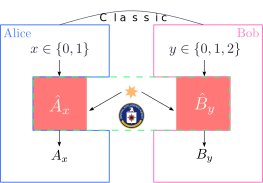
\includegraphics[width=0.95\textwidth]{chapters/deviceindependent/img/setup.pdf}
	\end{center}
	\caption{DIQKD Setup. Alice's lab (delimited by the blue line) and Bob's lab (delimited by the pink line) are linked by a classical channel of communication (gray cruved line), and by a quantum channel (green dashed rectangle). A source (yellow star) generated a state with one part sent to Alice while the other is sent to Bob. Alice selects an input $x$, to perform the measurement $\hat{A}_x$ and obtain the outcome $A_x$. Similarly Bob chose an input $y$, to measure with respect to $\hat{B}_y$ and obtain $B_y$.
	Eve, represented by the CIA logo, has full access to the quantum channel, and may have bloated the measurement devices. }
	\label{fig:DIQKD_setup}
\end{figure}

